\section{Support Vector Regression (SVR)}

\mode<presentation>{
\begin{frame} 
    \begin{center} \huge
        \secname
    \end{center}
    \begin{center}
    SVMs for regression problems   
    \end{center}
\end{frame}
}

\begin{frame}\frametitle{The classification setting}

\mode<article>{
The classification setting:\\
}

Classification problems have labels with only finite many possible values.

Example: Binary classification, $y_{T} \in \{-1,1\}$:

\begin{figure}[ht]
     \centering
     \savebox{\imagebox}{
	 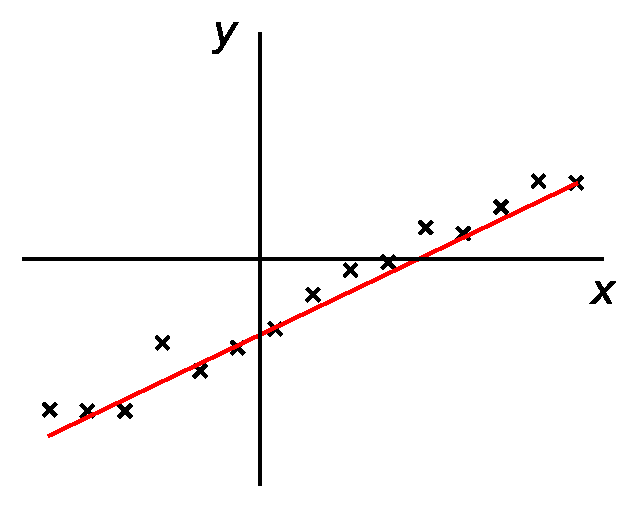
\includegraphics[width=0.35\textwidth]{img/classification_1d_sign}}%
     \begin{subfigure}[t]{0.35\textwidth}
         \centering
         \usebox{\imagebox}% Place largest image
         \caption{1D input}
         \label{fig:classification1d}
     \end{subfigure}
     \hspace{10mm}
     \begin{subfigure}[t]{0.35\textwidth}
         \centering
         \raisebox{\dimexpr.5\ht\imagebox-.5\height}{% Raise smaller image into place
         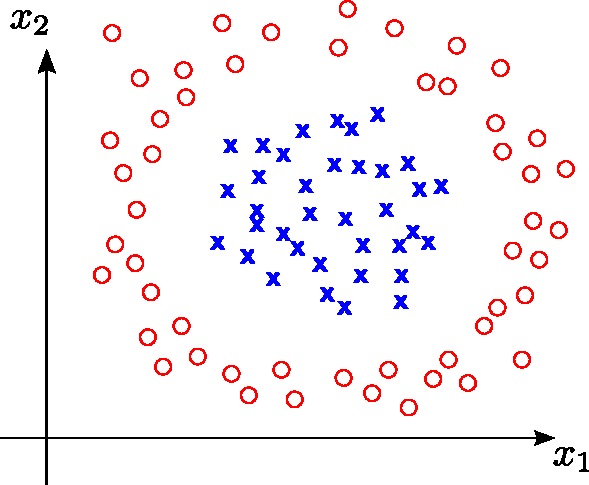
\includegraphics[width=0.99\textwidth]{img/circular}
         }
         \caption{2D input}
         \label{fig:classification2d}
     \end{subfigure}
     \caption{binary classification}
	 \label{fig:classification}
\end{figure}

\end{frame}

\begin{frame}\frametitle{Regression setting}

\mode<article>{
\underline{The Setting}:
}

\begin{itemize}
\item[] \underline{Data}:\\
    \begin{equation}
    \big\{ (\vec x^{(\alpha)}, y_{T}^{(\alpha)}\big\}_{\alpha=1}^{p}
    \end{equation}
    with $\vec x \in \R^{N}$ and $y_{T} \in \R${}

\item[] \underline{Model}:\\
    linear neuron:
    \begin{equation}
        y(\vec x; \vec w, b) = \vec w^{\top} \vec x + b
    \end{equation}


    
\end{itemize}


\begin{figure}[h]
     \centering
     \savebox{\imagebox}{
	 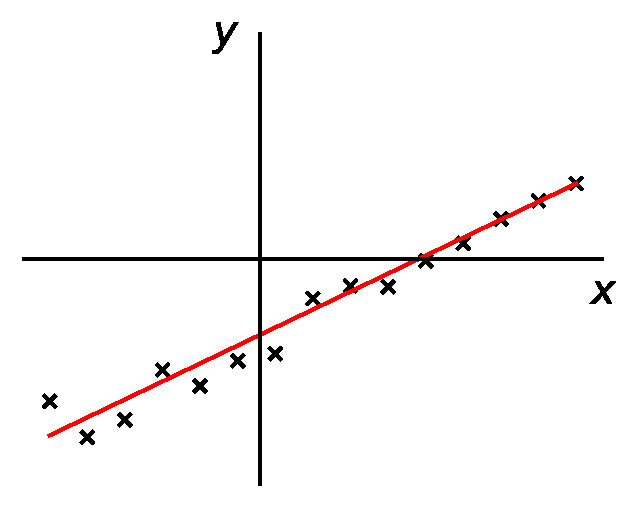
\includegraphics[width=0.35\textwidth]{img/regression_1d_linear}}%
     \begin{subfigure}[t]{0.35\textwidth}
         \centering
         \usebox{\imagebox}% Place largest image
         \caption{linear regression}
         \label{fig:regression1dlinear}
     \end{subfigure}
     \hspace{10mm}
     \begin{subfigure}[t]{0.35\textwidth}
         \centering
         \raisebox{\dimexpr.5\ht\imagebox-.5\height}{% Raise smaller image into place
         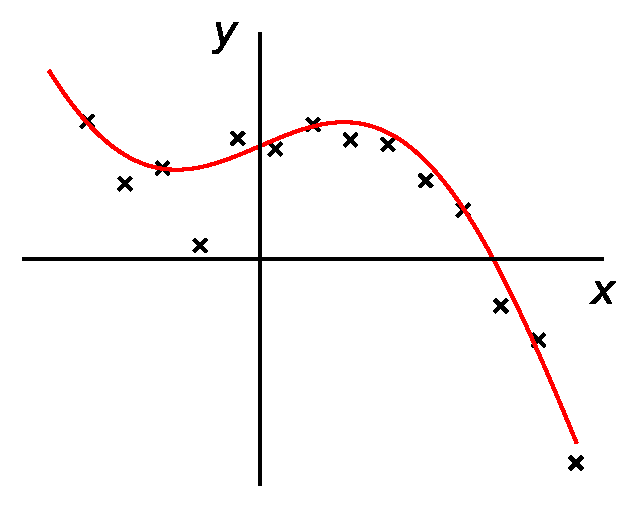
\includegraphics[width=0.99\textwidth]{img/regression_1d_nonlinear}
         }
         \caption{non-linear regression}
         \label{fig:regression1dnonlinear}
     \end{subfigure}
     \caption{scalar regression with 1D input}
	 \label{fig:regression}
\end{figure}



\end{frame}

\subsection{The $\epsilon$-sensitive cost function for regression}

\begin{frame}\frametitle{\subsecname}

\begin{equation}
e    
\end{equation}
    
\end{frame}
